\chapter{Evoluční algoritmy}
\section{Historie}
Začněme pohledem do historie Evolučních algoritmů na základě knih \cite{MitchellBook} a \cite{eibenIntro}. Darwinova myšlenka evoluce lákala vědce už před průlomem počítačů, Turing vyslovil myšlenku \textit{genetického a evolučního vyhledávání} už v roce 1948. V 50. a 60. letech nezávisle na sobě vznikají 4 hlavní teorie nesoucí podobnou myšlenku. Společným základem všech teorií byla evoluce populace kandidátů na řešení daného problému a jejich následná úprava způsoby hromadně nazývány jako genetické operátory, například mutace genů, přirozená selekce úspěšnějších řešení, atp.
\par 
Rechenberg a Schwefell (1965, 1973) představili \textit{Evoluční strategie}, což je metoda optimalizující parametry v reálných číslech, v jejich práci se objevují jako prostředek pro optimalizaci tvaru letadlových křídel. Fogel, Owens, Walsh zveřejnili \textit{evolutionary programming}(evoluční programování), technika využívající k reprezentaci kandidátů konečný automat (s konečným počtem stavů), který je vyvíjen mutací přechodů mezi stavy a následnou selekcí. \textit{genetické algoritmy} vynalezl Holand v 60. letech a následně se svými studenty a kolegy z Michiganské Univerzity vytvořil první implementaci. U genetických algoritmů, oproti ES a EP, nebylo hlavním cílem formovat algoritmus pro řešení konkrétních problémů, ale přenos obecného mechanismu evoluce jako metody aplikovatelné v informatickém světě. Princip GA spočívá v transformaci populace chromozomů (př. vektor 1 a 0) v novou populaci pomocí genetických operátorů křížení, mutací a inverze. V 1975 v knize \textit{Adaptation in Natural and  Artificial Systems} \cite{HolandBook} Holand definoval genetický algoritmus jako abstrakci biologické evoluce spolu s teoretickým základem jejich používání. Někteří vědci ovšem používají pojem GA i ve významech hodně vzdálených původní Holandově definici. K sjednocení jednotlivých přístupů přispěl v 90. letech John R. Koza, dále jsou všechny metody zahrnuty pod pojmem \textit{Evoluční algoritmy} jako jejich součásti. Dnes se věnuje tématu EA celá řada konferencí a odborných časopisů. Zmiňme ty nejvýznamnější z nich, v kontextu konferencí: 
\href{http://gecco-2017.sigevo.org/index.html/HomePage}{GECCO}, \href{http://www.ppsn2016.org/conference}{PPSN}, 
\href{http://www.cec2017.org/}{CEC}, 
\href{http://www.evostar.org/2018/}{EVOSTAR}, 
odborné časopisy časopisy, na které bych rád upozornil: 
\href{http://www.mitpressjournals.org/loi/evco}{Evolutionary Computation}, 
\href{http://ieeexplore.ieee.org/xpl/RecentIssue.jsp?reload=true&punumber=4235}{IEEE Transactions on Evolutionary Computation}, 
\href{http://www.springer.com/computer/ai/journal/10710}{Genetic Programming and Evolvable Machines},
\href{https://www.journals.elsevier.com/swarm-and-evolutionary-computation/}{Swarm and Evolutionary Computation}

\section{Co je evoluční algoritmus?}
Ač existuje mnoho variant evolučních algoritmů, jak jsme zmínili v krátké pohledu do historie, spojuje je společná myšlenka populace jedinců uvnitř prostředí s omezenými podmínkami. Jedinci, jinak také nazývání kandidáti, soutěží o zdroje daného prostředí, tím je docíleno přírodní selekce (přežijí jen ti nejlepší). Pokud budeme mít k dispozici kvalitativní funkci, kterou se snažíme maximalizovat, pak nebude problém vytvořit náhodné jedince z definičního oboru přesně této funkce. Náhodně vzniklé jedince můžeme ohodnotit, tímto způsobem dáme vzniknout abstrakci pro měření fitness (z anglického fit nejvhodnější, zapadající). Z vzniklých a ohodnocených jedinců lze zvolit ty nejlepší pro tvorbu nové generace jedinců. Tvorba nové generace probíhá kombinováním zvolených rodičů a mutacemi jedinců. Jako kombinaci uvažujeme operátor, který je aplikován na 2 a více zvolených kandidátů (proto se jim také říká rodiče) a tvořící 1 a více nových jedinců (také nazývány potomci). Mutace je aplikována pouze na jednoho jedince a její výsledkem je také pouze 1 jedinec. Tyto dvě operace aplikované na rodičovskou generaci vedou k vytvoření nových kandidátů (potomků, offsprings). I tato nová generace je ohodnocena fitness a dále soutěží se starými jedinci na základě fitness o místo v nové generaci, občas také mimo fitness funkce bereme v potaz stáří kandidáta. Popsaný proces je opakován dokud není nalezen kandidát s dostatečně velkou fitness nebo dosáhneme maximálního počtu iterací( bylo dosaženo požadovaného počtu opakovaní apod). Základy Evolučního systému pohání 2 základní hnací síly: variační operátory, selektivní operátory. Variační operátory zajišťují potřebnou různorodost v populaci a tím tvoří nové cesty k úspěšnému kandidátovi. Oproti tomu selektivní operátory zvyšují průměrnou kvalitu řešení v celé populaci. Kombinací těchto operátorů obecně vede ke zlepšování fitness hodnot v následující generaci. Celkem jednoduše lze pozorovat, zda evoluce optimalizuje či nikoliv, stačí nám k tomu pozorovat zda se fitness v populaci blíží více a více k optimálním hodnotám vzhledem k postupu v čase. Mnoho komponent zapříčiňuje, že EA se řadí ke stochastickým metodám, selekce totiž nevybírá nejlepší jedince deterministicky, i jedinci s malou fitness mají šanci být rodiči následující generace. Během kombinování jsou části rodičů, které budou z zkombinovány, také zvoleny náhodně. Podobně je tomu u mutací. Část která bude změněna, je taktéž určena náhodně, nové rysy nahrazující staré jsou generovány taktéž náhodně.  
\begin{center}
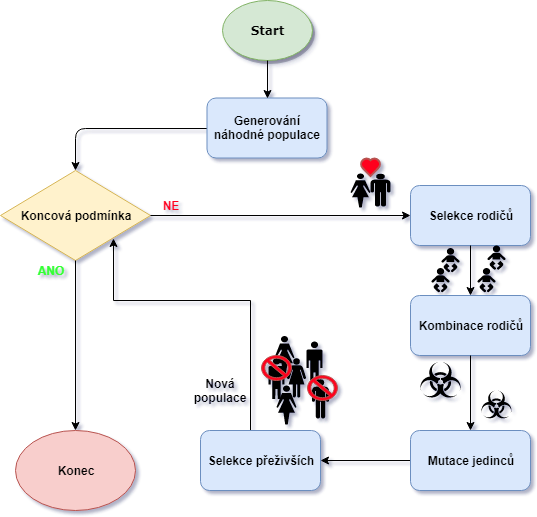
\includegraphics[scale=0.64]{../img/EA.png}
\end{center}
Ze schéma na obrázku můžeme vyčíst, že EA patří mezi algoritmy \"generate and test (vygeneruj a otestuj)\". Vyhodnocení fitness funkce poskytuje heuristický odhad kvality řešení, prohledávaní je řízen variací a selekcí. EA splňují charakteristické rysy G\&T algoritmů, zpracovávají zároveň celé kolekce kandidátů. Většina EA míchá informace ze 2 a více kandidátů. EA se řadí ke stochastickým metodám. \par
Různé dialekty evolučního programování, zmíněné v historickém okénku, splňují všechny tyto hlavní rysy. Liší se pouze v technických detailech. Kandidáti jsou často reprezentování různě, liší se datové struktury pro jejich uchování i jejich zakódování. Typicky se jedná o řetězce nad konečnou abecedou v případě GA, vektory reálných čísel v ES, konečné automaty v EP a stromy v GP. Důvod těchto rozdílů je hlavně historický. Technicky však lze upřednostnit jednu reprezentaci, pokud lépe odpovídá danému problému, tzn. kóduje kandidáta jednodušeji či přirozenější formou. Pro ilustraci zvolme řešení splnitelnosti(SAT) s n proměnnými, vcelku přirozeně sáhneme po použití řetězce bitů délky n a obsah i-tého bitu označuje, že i-tá proměnná má hodnotu (1)- pravda (0) - nepravda, proto bychom použili jako vhodný EA genetické algoritmy. Oproti tomu evoluce programu, který hraje šachy, by bylo vhodnější použít derivační strom, kde by vrcholy odpovídaly tahům na šachovnici. Přirozenější by tedy bylo použít GP. \par
Neopomeňme zmínit ještě dva důležité fakty. Za prvé kombinační a mutační operátory musí odpovídat dané reprezentaci, např. v GP kombinace pracuje se stromy (kombinuji podstromy..), zatímco v GA na řetězcích (prohazuji části řetězců). Za druhé oproti variacím musí fitness selekce záviset vždy pouze na fitness funkci, takže selekce pracuje nezávisle na reprezentaci.
\section{Části evolučních algoritmů}
Abychom vytvořili běhu schopný evoluční algoritmus, musíme specifikovat každou zmíněnou část a také inicializační funkci, která připraví první populaci. Pro konečný algoritmus ještě nesmíme opomenout a dodat koncovou podmínku. 
\begin{itemize}
\item{Reprezentace (definici individuí)}
\item{Ohodnocující funkce (Fitness funkce)}
\item{Populace}
\item{Selekce rodičů}
\item{Variační operátory (kombinace, mutace)}
\item{Selekce prostředí}
\end{itemize}
\subsection{Reprezentace}
Při tvorbě EA nejdříve musíme propojit prostor původního problému s prostorem řešení, kde se bude vlastní evoluce odehrávat. K docílení propojení je většinou potřeba zjednodušit či vytvořit abstrakci nad aspekty reálného světa (prostor problému), abychom vytvořili vhodný prostor řešení, kde mohou být jednotlivá řešení ohodnocena. Neboli chceme docílit, aby možná řešení mohla být specifikována a uložena, tak aby s nimi mohl počítač pracovat. Objekty reprezentující možná řešení v kontextu původního problému jsou nazývány \textbf{fenotyp}, zatímco kódování na straně EA prostoru se jim říká \textbf{genotyp}. Reprezentace označuje mapování z fenotypů na genotypy, používá se ve významu funkce z fenotypu na genotyp(encode) i genotypu na fenotyp(decode) a předpokládá se, že pro každý genotyp existuje nejvýše jeden fenotyp. Například pro optimalizační problém, kde množinou řešení jsou celá čísla. Celá čísla tvoří množinu fenotypu a můžeme se rozhodnout pro reprezentaci v binárních číslech. Tedy 18 by byl fenotyp a 10010 jeho genotyp. Prostor fenotypů a genotypů se zpravidla velmi liší a celý proces EA se odehrává pouze v genotypovém prostoru, vlastní řešení dostaneme rozkódováním nejlepšího genotypu po ukončení EA. Jelikož nevíme, jak vlastní řešení vypadá, je nanejvýš vhodné umět reprezentovat všechny možná řešení, v G\&T bychom řekli, že generátor je kompletní.
\begin{itemize}   
  \item V kontextu původního problému jsou následující výrazy ekvivalentní: fenotyp, kandidát(na řešení), jedinec, individuum (množina všech možných řešení = fenotypový prostor)
  \item V kontextu EA: genotyp, chromozom, jedinec, individuum (množina, kde probíhá EA prohledávání = genotypový prostor)
  \item Části individuí jsou nazývány gen, locus, proměnná a dále se dělí na alely, či hodnoty
  \end{itemize}
\subsubsection{Neuronové sítě} Pro reprezentaci jedinců v oblasti robotiky, rozpoznávání obrazů a dalších oblastí umělé inteligence se v poslední době používají nejčastěji neuronové sítě. Neuronová síť se strukturou podobá neuronovým sítím v mozku. Základní sítě se skládají z jednotlivých neuronů. V informatickém světě se jmenují perceptrony. Perceptron je funkce $\mathbb{R}^n \rightarrow \mathbb{R}$ a definovaná $\sum{i < n+1} w_{i} x_{i}$, kde pro $i < n$ $x_{i}$ je í-tý prvek vstupního vektoru, pro  $i == n$ je $x_{i}=1$. $w_{i}$ se označuje jako váha a většinou $w_{i} \in \mathbb{R}$. \par
Jednovrstvou neuronovou sítí pak myslíme n perceptronů, tedy funkci $\mathbb{R}^{n} \rightarrow \mathbb{R}^{n}$, kde í-tý prvek výstupního vektoru dostaneme aplikací i-té perceptronové funkce neuronové sítě. \par 
Pokud dovolíme skládání perceptronů, vzniknou nám tzv. vícevrstvé neuronové sítě. Podmnožiny výstupů z první vrstvy neuronů neurčují přímo výstup, ale jsou opět zvoleny jako vstupní vektory pro další jednovrstvou neuronovou síť. \par
Skrytá vrstva(hiden layer) je taková jednovrstvá neuronová síť, jejíž výstup je pouze vstupem jiné neuronové sítě. \par
\subsection{Populace}
Populace je multimnožina genotypů, slouží jako jednotka evoluce. Populace utváří adaptaci a změny, zatímco vlastní jedinci se nijak nemění, jen vznikají noví a nahrazují předešlé. Pro danou reprezentaci je definice populace velmi jednoduchá, charakterizuje ji pouze velikost. U některých specifických EA má populace další prostorové struktury, definované vzdáleností jedinců nebo relacemi sousedních jedinců, což by se dalo připodobnit reálným populacím, které se vyvíjejí v různých geografických prostředích. U většiny EA se velikost populace nemění, což vede k soutěživosti mezi jedinci(,zůstanou ti nejlepší). Na úrovni populací pracují právě selektivní operátory. Například zvolí nejlepší jedince aktuální populace jako rodiče následující a nahradí nejhorší jedince novými. Rozmanitost populace - vlastnost, které chceme z pravidel docílit, je měřena jako počet různých řešení v multimnožině. Neexistuje však jediné hledisko, podle kterého lze tuto vlastnost měřit, většinou se používá počet rozdílných hodnot fitness, rozdílných fenotypů či genotypů a také entropie(míra neuspořádanosti). Ovšem musíme mít na paměti, že jedna hodnota fitness v populaci neznamená, že populace obsahuje pouze jeden fenotyp, stejně tak jeden fenotyp nemusí odpovídat jednomu genotypu apod. 
\subsection{Selekce rodičů}
Rodičovská selekce, někdy také partnerská selekce, vybírá lepší jedince jako rodiče pro příští generaci. Jedinec se stává rodičem, pokud byl zvolen k aplikaci variačních operátorů a tím dal vzniknout novým potomkům. Společně s selekcí přeživších je rodičovská selekce zodpovědná za zvedání kvality v populacích. Rodičovská selekce je v EA většinou pravděpodobnostní metoda, která dává jedincům s větší kvalitou mnohem větší šanci býti vybrán než těm s nízkou. Nicméně i jedincům s nízkou kvalitou je často přidělena malá nenulová pravděpodobnost pro výběr, jinak by se celé prohledávání mohlo vydat slepou cestou a zaseknout se na lokální optimu. 
\subsection{Variační operátory}
Hlavní úlohou variačních operátorů(mutace, rekombinaci) je vytváření nových individuí ze starých. Z pohledu Generate  Test algoritmů spadají variační operátory do právě do Generate části. Obvykle je dělíme na dva typy podle jejich arity, jedná se o unární(Mutace) a n-arní(rekombinace) operátory.
\subsubsection{Mutace}
Ve většině případů myslíme unárním variačním operátorem mutace. Tento operátor je aplikován pouze na jeden genotyp a výsledkem je upravený potomek. Mutace řadíme mezi stochastické metody, výstup(potomek) totiž závisí na sérii náhodných rozhodnutí. Však mutace není vhodné pojmenování pro všechny variační operátory, například pokud se jedná o heuristiku závislou na daném problému, která se chová systematicky, hledá slabé místo a následně se jej snaží vylepšit, v tomto případě se nejedná o mutaci v pravém slova smyslu. Obecně by mutace měla způsobovat náhodné a nezaujaté změny. Unarní variační operátory hrají odlišnou roli v rozdílných EA opět díky historicky oddělenému vývoji. Zatímco v GP se nepoužívají vůbec, v GA mají velmi důležitou roli a v EP se jedná o jediný variační operátor. Díky variačním operátorům aplikovaným v jednotlivých evolučních krocích dostává prohledávací prostor topologickou strukturu. Existují teorie podporující myšlenku, že EA(s dostatečným časem) naleznou globální optimum daného problému opírající se právě o tuto topologickou strukturu a také spoléhají na fakt, že může vzniknout každý genotyp reprezentující možné řešení. Nejjednodušší cesta ke splnění těchto podmínek vede právě přes variační operátory. U mutací tohoto například dosáhneme, když povolíme, aby mohly skočit kamkoliv, tzn. každá alela může být zmutována na jakoukoli další s nenulovou pravděpodobností. Většina vědecké společnosti považuje tyto důkazy za nepříliš použitelné v praktickém využití a proto tuto vlastnost většina EA neimplementuje.  
\subsubsection{Rekombinace}
Rekombinace, také nazývána křížení, je binární variační operátor. Jak název napovídá, spojuje informace ze dvou rodičů(genotypů) do jednoho nebo dvou potomků. Stejně jako mutace patří rekombinace k stochastickým operátorům. Rozhodnutí, jaké části budou zkombinovány a jakým způsobem toho bude docíleno, závisí na náhodě. Role rekombinace se znovu liší v rozličných EA, v GP se jedná o jediné variační operátory, v EP nejsou použity vůbec. Existují  rekombinační operátory s vyšší aritou (, tzn.  používající více než 2 rodiče) a jsou také jednoduché na implementaci. Dokonce několik studií potvrdilo, že mají velmi pozitivní vliv na celou evoluci, ale nemají tak hojné zastoupení, nejspíše proto, že neexistuje biologický ekvivalent. Rekombinace funguje na jednoduchém principu, slučuje 2 individua a produkuje jednoho či více potomků, kteří kombinují jejich výhodné vlastnosti, tedy potomek by měl být úspěšnější než jeho rodiče. Tento princip podporuje fakt, že po 1000-letí se aplikací rekombinace na rostliny a zemědělská zvířata mnohokrát podařilo vytvořit nové jedince s vyšším výnosem či jinými výhodnými vlastnostmi(odolnost proti škůdcům atd). Evoluční algoritmy vytváří množství potomků náhodnou rekombinací a doufáme, že zatímco malá část nové generace bude mít nežádoucí vlastnosti, většina se nezlepší ani si nepohorší a konečně další malá část předčí jejich rodiče. Na naší planetě se sexuálně(kombinací dvou jedinců) rozmnožují pouze vyšší organismy, což vzbuzuje dojem, že rekombinace je nejvyšší forma reprodukce. Neopomeňme, že  variační operátory jsou závislé na reprezentaci(genotypu) jedinců. Např. pro genotypy bitových řetězců může použít bitovou inverzi jako vhodný mutační operátor bude-li ovšem genotyp strom musíme zvolit nějaký jiný. 
\subsubsection{Selekce prostředí}
Selekce prostředí, někdy také nazývána selekce přeživších, jak název napovídá má blízko k selekci rodičů, odlišuje jednotlivá individua na základě jejich fitness hodnoty. Oproti rodičovské selekci ji však používáme v jiné části evolučního cyklu. Selekci prostředí spouštíme hned po vytvoření nových potomků. Jelikož velikost populace kandidátů bývá skoro vždy konstantní, je nutné rozhodnout, které kandidáty zvolíme do další generace. Toto rozhodnutí většinou závisí na hodnotě fitness jednotlivých kandidátů, také se často hledí na dobu vzniku daného kandidáta. Dobou vzniku myslím generaci v které daný jedinec vznikl. Na rozdíl od rodičovské selekce, která bývá stochastická, bývá selekce prostředí deterministickou metodou. Uveďme dvě nejběžnější metody, obě kladou největší důraz na fitness. První vybírá nejlepší segment z množiny nových potomků i z původní generace nezávisle, druhá dělá totéž jen z množiny nových potomků. Selekce prostředí je uváděna i pod názvem \"záměnná\" strategie(replacement strategy). Selekce prostředí(přeživších) se víceméně používá, pokud je množina nových potomků větší než velikost generace a záměna využíváme když je nových potomků velmi málo.
\subsubsection{Inicializace populace}
Inicializace populace zastává důležitý úkol a to vytvořit první generaci kandidátů. Její implementace bývá ve většině EA její implementace velmi jednoduchá. První generace je vygenerována čistě náhodně. Principiálně by se zde dalo využít nějaké heuristiky k vytvoření vyšší fitness v první generaci, ovšem musela by zohledňovat řešený problém. Jestli tento postup stojí za výpočetní čas, velmi záleží na konkrétní aplikaci EA. Ovšem existují obecná doporučení, která se touto otázkou zabývají. 
\subsubsection{Ukončovací podmínka}
Rozlišme dvě varianty vhodné ukončovací podmínky. Pokud řešený problém má známou optimální hodnotu fitness, potom v ideální případě ukončovací podmínkou je řešení s touto fitness. Pokud jsme si vědomi, že náš model oproti modelovanému prostředí obsahuje nutná zjednodušení nebo by se v něm mohly vyskytovat nežádoucí šumy, lze se spokojit s řešením, které dosáhlo optima fitness s přesností $\epsilon > 0$. Nicméně, EA díky své stochastičnosti většinou nemohou garantovat dosažení takovéto hodnoty fitness, takže ukončovací podmínka by nemusela být nikdy splněna a algoritmus by běžel věky. Kdybychom vyžadovali konečnost algoritmu, musíme rozšířit ukončovací podmínku. Zatím-to účelem se nejběžněji používají následující rozšíření: \par
\begin{enumerate}
\item Byl překročen čas vyhrazený pro počítání na CPU
\item Celkový počet evaluací fitness přesáhl svůj předem daný limit 
\item Zlepšení fitness v dané časovém bloku(měřenému počtem generací, či evaluací) klesla pod přípustný práh.
\item Rozmanitost v populaci nedosahuje předem určených hodnot
\end{enumerate}
Ukončovací podmínka bývá prakticky disjunkce následujících tvrzení: dosáhli jsme optima or podmínka X ze seznamu. Může se stát, že optimum známé není. Pak se používá pouze zmíněných podmínek nebo se smíříme s nekonečností algoritmu. 

\section{Diferenciální evoluce}
Diferenciální evoluce(DE) se objevila v roce 1995, kdy Storn a Price vydali technický report \cite{Storn1997}. Tento evoluční algoritmus popíši trochu více, protože je jedním z klíčových algoritmů mého řešení. 
\subsubsection{Charakteristické vlastnosti}
DE dostala své jméno hlavně díky změnám obvyklých reprodukčních operátorů v EA. Diferenciální mutace, jak jsou mutace v DE nazývány, z dané populace kandidátů vektorů v $\mathbb{R}^n$ vzniká nový mutant $\overline{x}'$ přičtením pertubačního vektoru(pertubation vector) k existujícímu kandidátovi. \par
$\overline{x}'=\overline{x}+\overline{p}$ \par
Kde pertubační vektor $\overline{p}$ je vektor rozdílů dvou náhodně zvolených kandidátů z populace $\overline{y} a \overline{z}$. \par 
$\overline{p}=F\dot(\overline{y}-\overline{z})$ \par
Škálovací faktor $F>0$, $F \in \mathbb{R}$, který kontroluje míru mutace v populaci. Jako rekombinační operátor v DE slouží uniformní křížení, pravděpodobnost křížení je dána $C_r \in [0,1]$, definuje šanci jakékoli pozice v rodiči, že odpovídající allela potomka bude brána z 1. rodiče. DE také upravuje křížení, neboť 1 náhodná allela je brána vždy z 1. rodiče, aby nedocházelo k duplikaci 2. rodiče. \par 
V hlavních implementacích DE reprezentují populace spíše listy, odpovídají lépe než množiny, umožňují referenci i-tého jedince podle pozice $i\in{1,..,\mu}$ v listu. Pořadí kandidátů v této populaci $P=<\overline{x_1}...\overline{x_i}...\overline{x_{\mu}}>$ není závislé na hodnotě fitness.Evoluční cyklus začíná vytvořením populace vektorů mutantů $M=<\overline{v_1}...\overline{v_{\mu}}>$. Pro každého nového mutanta $\overline{v_i}$ jsou zvoleny 3 vektory z P, base vektor a dva definující pertubační vektor. Po vytvoření populace mutantů V, pokračujeme tvorbou populace $T=<\overline{u_1},....\overline{u_{\mu}}>$, kde $\overline{u_i}$ je výsledek aplikace křížení $\overline{u_i}$ je výsledek křížení $\overline{v_i}$ a $\overline{x_i}$(všimněme si, že je zaručené, že nezreplikujeme $\overline{x_i}$). Jako poslední aplikujeme selekci na každý pár $\overline{x_i}$ a $\overline{u_i}$ a do další generace vybereme $\overline{u_i}$ pokud $f(\overline{u_i}) \leq f(\overline{x_i})$ jinak $\overline{x_i}$. \par 
DE algoritmus upravují 3 parametry, ?scalovací? faktor F, velikost populace $\mu$ (obvykle značen NP v DE literatuře) a pravděpodobnost křížení $C_r$. Na $C_r$ lze také pohlížet jako na míru mutace, tzn. allela nebude odděděna od mutanta.\par

\begin{center}
\begin{tabular}{ l l }
    \multicolumn{2}{c}{Vlastnosti Differciální Evoluce:} \\
    \hline \hline
    Reprezentace: & vektor $\mathbb{R}^n$ \\
    \hline  
    Rekombinace: & uniformní křížení \\
    \hline  
    Mutace: & differeční mutace \\
    \hline   
    Rodičovská selekce: & uniformní náhodné selekce 3 nezbytných vektorů \\
    \hline   
    Selekce prostředí: & deterministická selekce elity (dítě vs rodič) \\
  \end{tabular}
\end{center} \par
\subsubsection{Varianty DE:}
Během let, vzniklo a bylo publikováno mnoho variant DE. Jedna z modifikací zahrnuje možnost base vektoru, když vytváříme mutantské populace M. Může být náhodně zvolen pro každé $v_i$, jak bylo řečeno, ale také lze využít jen nejlepšího vektoru a nechat změny na pertubačním vektoru. Další možnost otevírá použití více pertubačních vektorů v mutačním operátoru. Což by vypadalo následovně: \par
$\overline{p} = F (\overline{y}-\overline{z} + \overline{y}' - \overline{z}')$, kde $\overline{y}, \overline{z}, \overline{y}',\overline{z}'$ jsou náhodně vybrány z původní populace.\par
Abychom odlišili různé varianty, používá se následující notace DE/a/b/c, kde \textbf{a} specifikuje base vektor(rand, best), \textbf{b} specifiuje počet differečních  vektorů při vzniku pertubačního vektoru, \textbf{c} značí schéma křížení (bin=uniformní). Takže podle této notace by základní verze DE byla zapsána takto: DE/rand/1/bin. 
\section{Evoluční strategie}
Evoluční strategie(Evolution Strategies) byly představeny na počátku 60. let pány Rechenbergem a Schwefelem \cite{Beyer2002}, oba jmenovaní pánové se zabývali optimalizací tvarů křídel na Technické univerzitě v Berlíně. Jedná se o evoluční algoritmus cílící na optimalizaci vektorů reálných čísel. Objevili si dvě schémata (1+1) a (1,1). Starší (1+1) (one plus one ES) vytvářejí potomka mutací a to přičtením náhodných nezávislých hodnot ke složkám rodičovského vektoru, následně je potomek přijat, pokud získal lepší fitness než jeho rodič. Jako další vznikl (1,1) (one comma one ES), které neimplementovalo elitismus, tzn. měnila vždy rodiče potomkem. Mutační funkce bere náhodná čísla z Normálního rozdělení s se střední hodnotou 0 a odchylkou $\sigma$. $\sigma$ se také nazývá velikost mutačního operátoru(mutation step size). Vylepšení původního algoritmu bylo představeno v 70. letech, jedná se o koncept multisložkových ES, které se skládají ze $\mu$ jedinců(velikost populace) a $\lambda$ jedinců vygenerovaných během jednoho cyklu. Opět tento koncept existuje ve 2 verzích $(\mu,\lambda)$ a $(\mu + \lambda)$. Zatímco bežné rekombinační schéma zahrnuje dva rodiče a jednoho potomka, intermediate křížení, které se u ES používá, zprůměruje hodnoty z rodičovských alel. Tímto způsobem můžeme používat i rekombinační operátory s použitím více než 2 rodičů, tyto operátory se nazývají globalní rekombinace. Konkrétně se na potomkovi podílí $\lambda$ rodičů. V praxi se preferuje $(\mu,\lambda)$ před $(\mu + \lambda)$, protože zahazuje všechny rodiče, tím pádem se snadno nezastaví na lokálním optimu, $(\mu,\lambda)$ se zvládá lépe adaptovat i při hledání pohyblivého optima. Pro typické použití se používá poměr 1:4 a 1:7. 
\begin{center}
  \begin{tabular}{ l l }
      \multicolumn{2}{c}{Vlastnosti Evolučních strategií:} \\
      \hline \hline
      Reprezentace: & vektor $\mathbb{R}^n$ \\
      \hline  
      Rekombinace: & intermediary křížení \\
      \hline  
      Mutace: & přičítání náhodných hodnot z norm. rozdělení \\
      \hline   
      Rodičovská selekce: & uniformní náhodná \\
      \hline   
      Selekce prostředí: & (sigma,lambda) nebo (sigma + lambda) \\
    \end{tabular} 
  \end{center} \par
  Násladuje krátký jednoduchý příklad ES v jazyku Pythonu, pro lepší pochopení jsem použil kód ze stránky \citep{openAiEs}. Cílem tohoto velmi jednoduché programu je nalézt vektor čísel, který se co nejvíce blíží vektoru solution
  \lstset{language=Python}
  \begin{lstlisting}[frame=single]  % Start your code-block
    import numpy as np
    solution = np.array([0.5, 0.1, -0.3])
    #fitness funkce, kter pocita vzdalenost
    #mezi vlozenym vektorem a solution 
    def f(w): return -np.sum((w - solution)**2)
    
    npop = 50     
    sigma = 0.1    
    # learning rate
    alpha = 0.001  
    w = np.random.randn(3)
    for i in range(300): 
    # vygenerujme npop mutaci k aktualnimu reseni
      N = np.random.randn(npop, 3) 
      # vektor R slouzi k uchovani fitness hodnot
      R = np.zeros(npop) 
      # Pro kazdou vyrobenou mutaci
      for j in range(npop): 
      # Aplikujeme mutaci na aktualniho jedince
        w_try = w + sigma*N[j]
        # Ohodnotime uspesnost zmutovaneho jedince 
        vzhledem k fitness funkci
        R[j] = f(w_try) 
      A = (R - np.mean(R)) / np.std(R) 
      # upravime aktualni reseni mutacemi, 
      # cim uspesnejsi mutace, 
      # tim vetsi vliv do aktualniho jedince.

      w = w + alpha/(npop*sigma) * np.dot(N.T, A)  
     \end{lstlisting}
